\section{Auditory System}
The term \textit{auditory system} refers to the sensory system for the perception of sound. In context with the given project, an overview of the paths, on which sound waves reach the nerve cells on the basilar membrane. There are two general principles: the \gls{ac} and \gls{bc}. Airborne waves lead to cochlea stimulation by moving the tympanic membrane whereas boneborne sound is stimulating the cochlea through vibrations of the skull. The pathway for airborne sound, which lead from the pinna, through the ear canal to the tympanic membrane and through the middle ears to the basilar membrane in the cochlea has been studied extensively and is regarded to be well known. Opposed to this, the details of \gls{bc} have not been investigated entirely \citep{stenfelt_2005} and are the subject of recent studies. The following section will outline both the \gls{ac} and \gls{bc} hearing.


\section{Air conduction of sound}
The typical way to stimulate the nerve cells on the basilar membrane and therefore perceive sound, is via \gls{ac}. The pathway from airborne wave outside the ear to the cochlea can be divided into three sections. In the first section, the sound wave is travelling through the outer ear, which consists of the pinna and the ear canal. The second section is comprised by the middle ear, where the so called Tympanic membrane, that seperates the middle ear and the outer ear, converts airborne waves into mechanical movement. The middle ear consists of three auditory bones (\textit{ossicles}) and is joined by the Eustachian tube. One of the ossicles is connected to the Tympanic membrane and another ossicle is connected to the oval window. The remaining ossicle connects formerly mentioned ones. The third section is within the inner ear. The oval window, that is set into motion by the ossicles in the middle ear, transfers the motion into a fluid-borne wave \citep{ho_2017}. The inner ear consists of the cochlea and the vestibular system. The latter is a system for equilibrioception and does not have any influence on hearing. For the hearing only the cochlea is of interest in the inner ear. The following \autoref{fig:hearing_system} shows the formerly described parts of the auditory system.


 \begin{figure}[H]
	\centering
		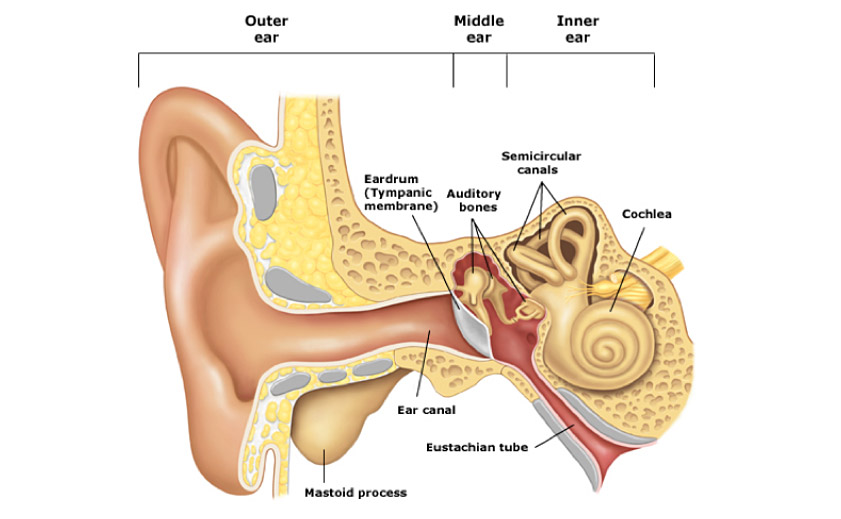
\includegraphics[width=1\textwidth]{anatomy-of-ear.jpg}
		\caption{The figure shows the outer ear, the middle ear and the inner ear.}
		\label{fig:hearing_system}
\end{figure}

\subsection{Functions of ear parts}
The pinna of the outer ear is shaped differently for every person and is very important for localisation of sound event. The shape of the pinna makes amplification, peaks and dips in the sound wave and including the ear canal the changing of the sound in the outer ear is called the \gls{hrtf}. Since the pinna is different for every person, every person have there own \gls{hrtf} and the brain have learned from birth the exact \gls{hrtf}. By changing the \gls{hrtf} on a person, the brain will be confused, but with time the brain can learn a new \gls{hrtf} if necessary. After the sound waves have entered the outer ear and changed by the pinna and the ear canal the tympanic membrane, also called the eardrum, is moving accordingly to the air pressure variation in the ear canal and transmitted to the middle ear.  

The middle ear consist of the three auditory bones, the hammer (malleus), the anvil (incus) and the stirrup (stapes), where the sound wave is travelling mechanically. The bone act as a impedance adaptation from air to liquid and have an amplification of approximation 20 times. The Eustachian tube function is to equalise the air pressure on both side on the eardrum. A build up pressure in the middle ear will affect the hearing negatively. The bone Mallus is attached to the oval window where stapes is attached to the tympanic membrane.

Vibration of the oval window cause wave travelling in the cochlea fluids, those fluid borne wave makes the basilar membrane to vibrate because pressure difference between the cochlear perilymphatic \citep{ho_2017}. The vibration of the basilar membrane gets the inner hair cell to move and generate electric response signal that is transmitted through the auditory nerve to the brain.



\section{Bone conduction of sound}\label{sec:bonepaths}
At the moment there is not a general delimited definiton of what \gls{bc} means, but it is mostly accepted as the sound transmission through the bones of the skull. However, \gls{bc} is not only limited to bones, since it usually also involves transmission through soft tissue and cartilage. Therefore, it can be identified as the transmission of sound energy through the body (bones, soft tissue and cartilage). 
\gls{bc}, although being performed in a localised way, involves the outer, middle and inner ear, as well as the bones surrounding the hearing apparatus and both its fluids and cerebrospinal fluid (CSF) \citep{puria_2013}.
 \begin{figure}[H]
	\centering
		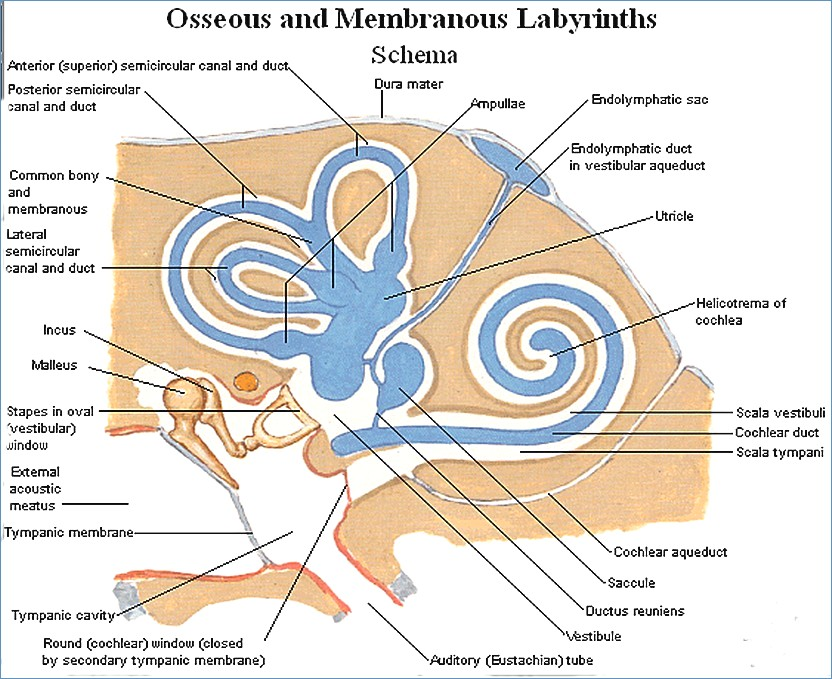
\includegraphics[width=1\textwidth]{more-on-the-vestibular-system-of-anatomy-of-cochlear-aqueduct.jpg}
		\caption{The figure shows the outer ear, the middle ear and the inner ear in detail}
		\label{fig:hearing_system_detail}
\end{figure}
Stenfelt's section 6.1.1 of \citep{puria_2013},starts with the following quote: \enquote{One of the quintessential questions about BC hearing is the end organ for
transforming BC vibration in the skull to neural code}. From this quote, we can infere that the determination of the endpoint for \gls{bc} is not an easy task, and could be the pinnacle in fully understanding \gls{bc} sound transmission.

As explained throughout the referenced section, several studies and experiments have been conducted over the years, leading to the result of identifying the cochlea as such organ. Once the endpoint was identified, it was primordial to understand the ways in which the sound is propagating to reach it.
\subsection{Propagation factors}

When analysing \gls{bc} propagation, we have to take into account three main factors:

\begin{itemize}
\item \textbf{Frequency}: there have been several studies and experiments over time both focused and skull and cochlea vibration patterns. These studies have served as ground for identifying four main modes within the human skull vibration pattern for frequencies below \SI{10}{\kilo\hertz}.
\begin{enumerate}
\item Below \SI{400}{\hertz}: within this range the skull moves as a rigid body (Fig \ref{fig:skull_vibration_pattern}a).\citep{stenfelt_2005b}
\item Between \SI{400}{\hertz} and \SI{1}{\kilo\hertz}: within this range the skull's motion can be described as a mass-spring system(Fig \ref{fig:skull_vibration_pattern}b).
\item Between \SI{1}{\kilo\hertz} and \SI{2}{\kilo\hertz}: at \SI{1}{\kilo\hertz}, the first free resonance of the skull appears \citep{hakansson_1994} and the motion transitions from mass-spring system to a system dominated by wave transmission.
\item Above \SI{2}{\kilo\hertz}: when reaching this range, wave transmission dominates the skull vibration pattern completely, with differences between the cranial vault and the skull base (Fig \ref{fig:skull_vibration_pattern}c).
\end{enumerate}
\begin{figure}[H]
	\centering
		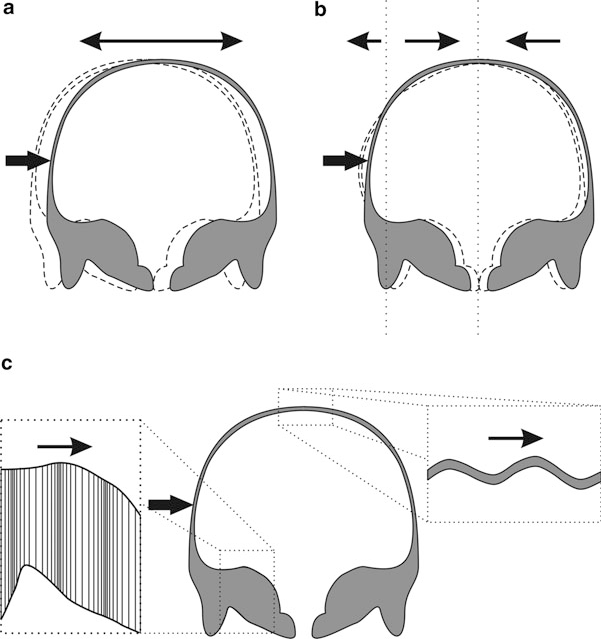
\includegraphics[width=1\textwidth]{skull_vibration_pattern.pdf}
		\caption{Two-dimensional illustration of the vibration modes of the human skull at frequencies between 0.1 and 10 kHz. The thick arrows indicate the stimulation position and the thin arrows indicate the response directions. The rigid body response at the lowest frequencies is illustrated in (a) while the response at frequencies between approximately 0.3–1.0 kHz that is similar to a massspring system is shown in (b) where three sections of the skull move sequentially in opposite directions. In (c) the vibration responses for frequencies above 2 kHz is illustrated differently for the skull base and the cranial vault: at the skull base longitudinal wave propagation dominates the response while a mixture of vibration modes including bending waves is present at the cranial vault \citep{puria_2013}}
		\label{fig:skull_vibration_pattern}
\end{figure}
\item \textbf{Skin and soft tissue}: generally, \gls{bc} transducers are placed pressed on skin-covered bone, meaning that the sound transmission will be affected by the presence of skin and soft tissue between the transducer and the bone. This often means that the sound transmission is attenuated when the skin is present, with an increase of up to \SI{20}{\decibel} in the acceleration threshold level \citep{hakansson_1985}.
\item \textbf{Position of the transducer}: the stimulation area is one of the key points in terms of increasing the sensitivity of \gls{bc} sound. This increase in sensitivity can be obtained by positioning the stimuli closer to the cochlea, which usually leads to the mastoid being selected as stimulation area. The reason for the improved sensitivity in this area could be related to the in-line position of the bone with regards to the petrous bone encapsulating the cochlea, or it could involve any of the skull bone structures \citep{puria_2013}. Therefore, further testing will be performed in order to identify the best position for our study case.
\end{itemize}
\subsection{Influence of Inner/Middle/Outer ear}

Early theories suggested that there were just a couple of pathways dominating the \gls{bc} perception. However, more recent studies suggest that there are five reported pathways for sound vibration to propagate or transmit to the cochlea \citep{zhang_2016}:
\begin{enumerate}
\item External auditory canal sound radiation (outer ear).
\item Inertia of the ossicular chain (middle ear).
\item Inertia of the cochlear fluid (inner ear).
\item Cochlear walls' compression (inner ear).
\item CSF pressure (inner ear).
\end{enumerate}

These pathways can work independently, but all of them add up to the quality of the signal received by the cochlea, and a failure in one of the pathways leads to a decrease in the quality of the received stimuli. In figure \ref{fig:hearing_system_pathway}, this correlation between \gls{bc} and \gls{ac} stimuli is depicted, clearly showing how \gls{bc} stimulation can generate \gls{ac}-like responses in the outer, middle and inner ear.

 \begin{figure}[H]
	\centering
		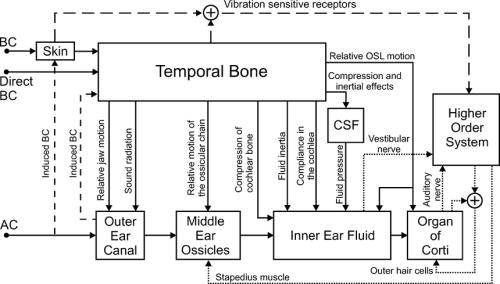
\includegraphics[width=1\textwidth]{ovidweb}
		\caption{The figure shows the transmission path for \gls{bc} \citep{stenfelt_2005}}
		\label{fig:hearing_system_pathway}
\end{figure}

\subsection*{Outer ear}

The outer ear consists of the pinna and the ear canal, meaning that half its structure is surrounded by cartilage and half by bone. When using \gls{bc} stimulation, sound pressure is produced in the ear canal due to vibration transmission in the ear canal walls. This sound pressure is transmitted to the cochlea in a similar way as \gls{ac} sound does, meaning that the \gls{bc} component of the outer ear needs to go through the middle ear before reaching the cochlea. The frequency response of the ear canal, as well as the sound pressure generated inside it can be manipulated by, for example, occlusion of the ear canal. In order to test the importance of the ear canal sound pressure, and as explained in \citep{puria_2013}, is to compare the sound pressure generated during \gls{bc} and \gls{ac} stimulation for the same sensation for an open ear canal. The result of this test lead to observe that above \SI{0.5}{\kilo\hertz} \gls{ac} stimulation generated greater sound pressure. After several other studies, it has been concluded that the ear canal sound pressure is not the dominant contributor for \gls{bc} sound.

\subsection*{Middle ear}

The middle ear is the portion of the ear between the eardrum and the oval window of the inner ear. It consists of three ossicles (maellus, incus and stapes), the tympanic cavity and the Eustachian tube. The middle ear contributes to \gls{bc} sound perception by transmission through ossicular inertia and sound pressure in the tympanic cavity. The influence of the middle ear ossicles on \gls{bc} has been thoroughly studied and references can be found in section 6.5 of \citep{puria_2013}, and it widely varies depending on the frequency range and on the status of the middle ear ossicles themselves.

\subsection*{Inner ear}

The inner ear is the innermost part of the ear, composed by the cochlea and the vestibular system. As stated previously, the cochlea is the end-organ for \gls{bc} sound transmission, and therefore will be the endpoint for all \gls{bc} transmission components or pathways. The inner ear is the dominating component for \gls{bc} sound perception, and although the middle and outer ear are also involved in the transmission, their effect on \gls{bc} sensitivity is very little compared to the inner ear. This is the main reason why \gls{bc} tresholds are compared with \gls{ac} tresholds in audiology in order to diagnose conductive impairment. However, there is still an ongoing debate over the exact processes that result in cochlear's \gls{bc} sound perception. Some of the major recent theories can be found in section 6.3.3 of \citep{puria_2013}.
